\documentclass[tikz,border=5pt]{standalone}
\usetikzlibrary{positioning,decorations.pathreplacing}
\begin{document}
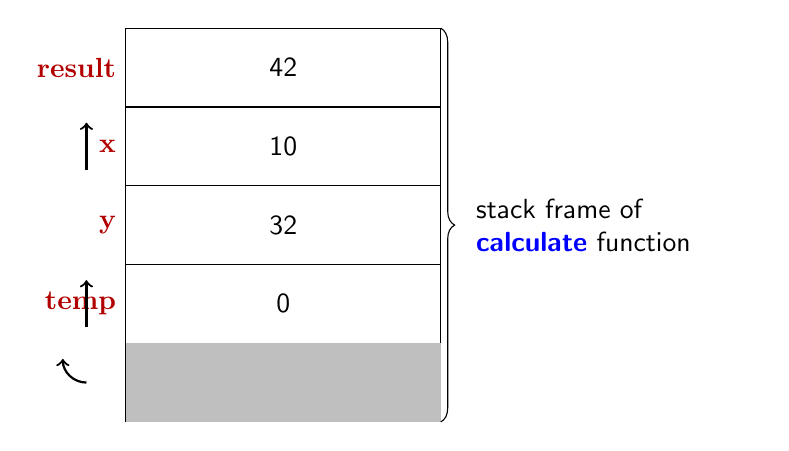
\begin{tikzpicture}[font=\sffamily]
  % Draw the stack rectangles
  \draw (0,0.0) rectangle (4.0,-1.0);
  \draw (0,-1.0) rectangle (4.0,-2.0);
  \draw (0,-2.0) rectangle (4.0,-3.0);
  \draw (0,-3.0) rectangle (4.0,-4.0);
  \draw (0,-4.0) rectangle (4.0,-5.0);

  % Fill gray areas
  \fill[gray!50] (0,-4.0) rectangle (4.0,-5.0);

  % Labels inside rectangles
  \node at (2.0,-0.5) {42};
  \node at (2.0,-1.5) {10};
  \node at (2.0,-2.5) {32};
  \node at (2.0,-3.5) {0};
  \node at (2.0,-4.5) {};

  % Variable names on left
  \node[anchor=east, text=red!70!black, font=\bfseries] at (0,-0.5) {result};
  \node[anchor=east, text=red!70!black, font=\bfseries] at (0,-1.5) {x};
  \node[anchor=east, text=red!70!black, font=\bfseries] at (0,-2.5) {y};
  \node[anchor=east, text=red!70!black, font=\bfseries] at (0,-3.5) {temp};

  % Arrows on left side
  \draw[->, thick] (-0.5,-1.8) -- (-0.5,-1.2);
  \draw[->, thick] (-0.5,-3.8) -- (-0.5,-3.2);
  \draw[->, thick] (-0.5,-4.5) arc(-90:-180:0.3);

  % Bracket for annotation
  \draw[decorate,decoration={brace,amplitude=5pt,mirror}]
    (4.0,-5.0) -- (4.0,0) node[midway,xshift=2.2cm,text width=3.5cm,align=left]
    {stack frame of \\ \textit{\textbf{\textcolor{blue}{calculate}}} function};

\end{tikzpicture}
\end{document}